\documentclass{article}
\usepackage{tikz}
\usetikzlibrary{shadows}
\begin{document}

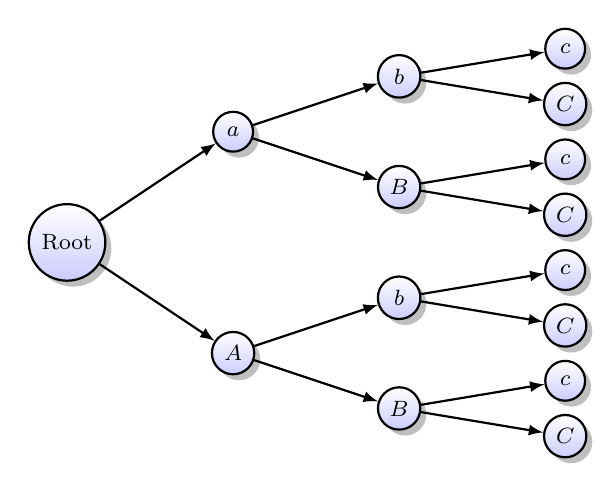
\begin{tikzpicture}[
level distance = 6em,
left/.style = {edge from parent/.style={>=latex, <-, thick, draw}},
right/.style = {edge from parent/.style={>=latex, ->, thick, draw}},
sloped,
root/.style = {font=\footnotesize, thick, shape=circle,
    draw, align=center, drop shadow,
    top color=white, bottom color=blue!20},
next/.style = {font=\footnotesize, text width=4mm, inner sep=1pt, thick, shape=circle,
    draw, align=center, drop shadow,
    top color=white, bottom color=blue!20},
level 1/.style={sibling distance=8em},
level 2/.style={sibling distance=4em},
level 3/.style={sibling distance=2em}
]

\node[root] {Root}[grow=0,right] %<-
  child{node[next] {$A$}
    child{node[next] {$B$}
      child{node[next] {$C$}}
      child{node[next] {$c$}}}
    child{node[next] {$b$}
      child{node[next] {$C$}}
      child{node[next] {$c$}}}}
  child{node[next] {$a$}
    child{node[next] {$B$}  
      child{node[next] {$C$}}
      child{node[next] {$c$}}}
    child{node[next] {$b$}
      child{node[next] {$C$}}
      child{node[next] {$c$}}}}
;
\end{tikzpicture}
\end{document}
